% this file is called up by thesis.tex
% content in this file will be fed into the main document

\chapter{Introduction}
\label{cha:intro}

Perhaps the most elusive subatomic particle known to science is the
Neutrino. With no electrical charge (thus aptly named) and mass
smaller than any other elementary particles, neutrinos simply pass
through other matter making them virtually undetectable. However,
neutrinos are sought after by researchers especially the ones working
in the fields of Astrophysics and Astronomy since they may help us
gain insights into astronomical events such as the birth of a neutrino
star or a supernova.

When neutrinos experience a change in the density of the matter they
are passing through(such as going from air into water), they
experience a change in velocity thus emitting an electron and a
photon. This phenomenon is known as Cherenkov Radiation
\cite{margiotta2014km3net} and is an indirect method which can be used
to detect neutrinos. In fact, this remains the premise for some of the
worlds largest neutrino observatories built to date such as the
Sudbury Neutrino Observatory (Ontario, Canada), The Super-Kamiokande
(Gifu Prefecture, Japan) and The IceCube Neutrino Observatory
(Antarctica).

The KM3NeT or the Cubic Kilometer Neutrino Telescope is the next
generation neutrino telescope, currently being constructed at the
bottom of the Mediterranean Sea. The goal of this research
infrastructure is two fold. First, is to study high energy neutrinos
originating from celestial events in the galaxy. And second, to study
the properties of the neutrino particles produced in the Earth's
atmosphere \cite{adrian2016letter}. The first goal will be realized
with the KM3NeT/ARCA (Astroparticle Research with Cosmics in the
Abyss) telescope and the second with KM3NeT/ORCA (Oscillation Research
with Cosmics in the Abyss) \cite{adrian2016letter}. In this paper, we
talk exclusively about KM3NeT/ARCA.

\begin{figure}[htb]
  \centering
  \begin{minipage}{0.74\textwidth}
    \includegraphics[width=\linewidth]{blocks.jpg}
    \caption{Artist's impression of the ARCA detector \textit{source: https://www.km3net.org}}%
    \label{fig:blocks}    
  \end{minipage}
  \begin{minipage}{0.24\textwidth}
    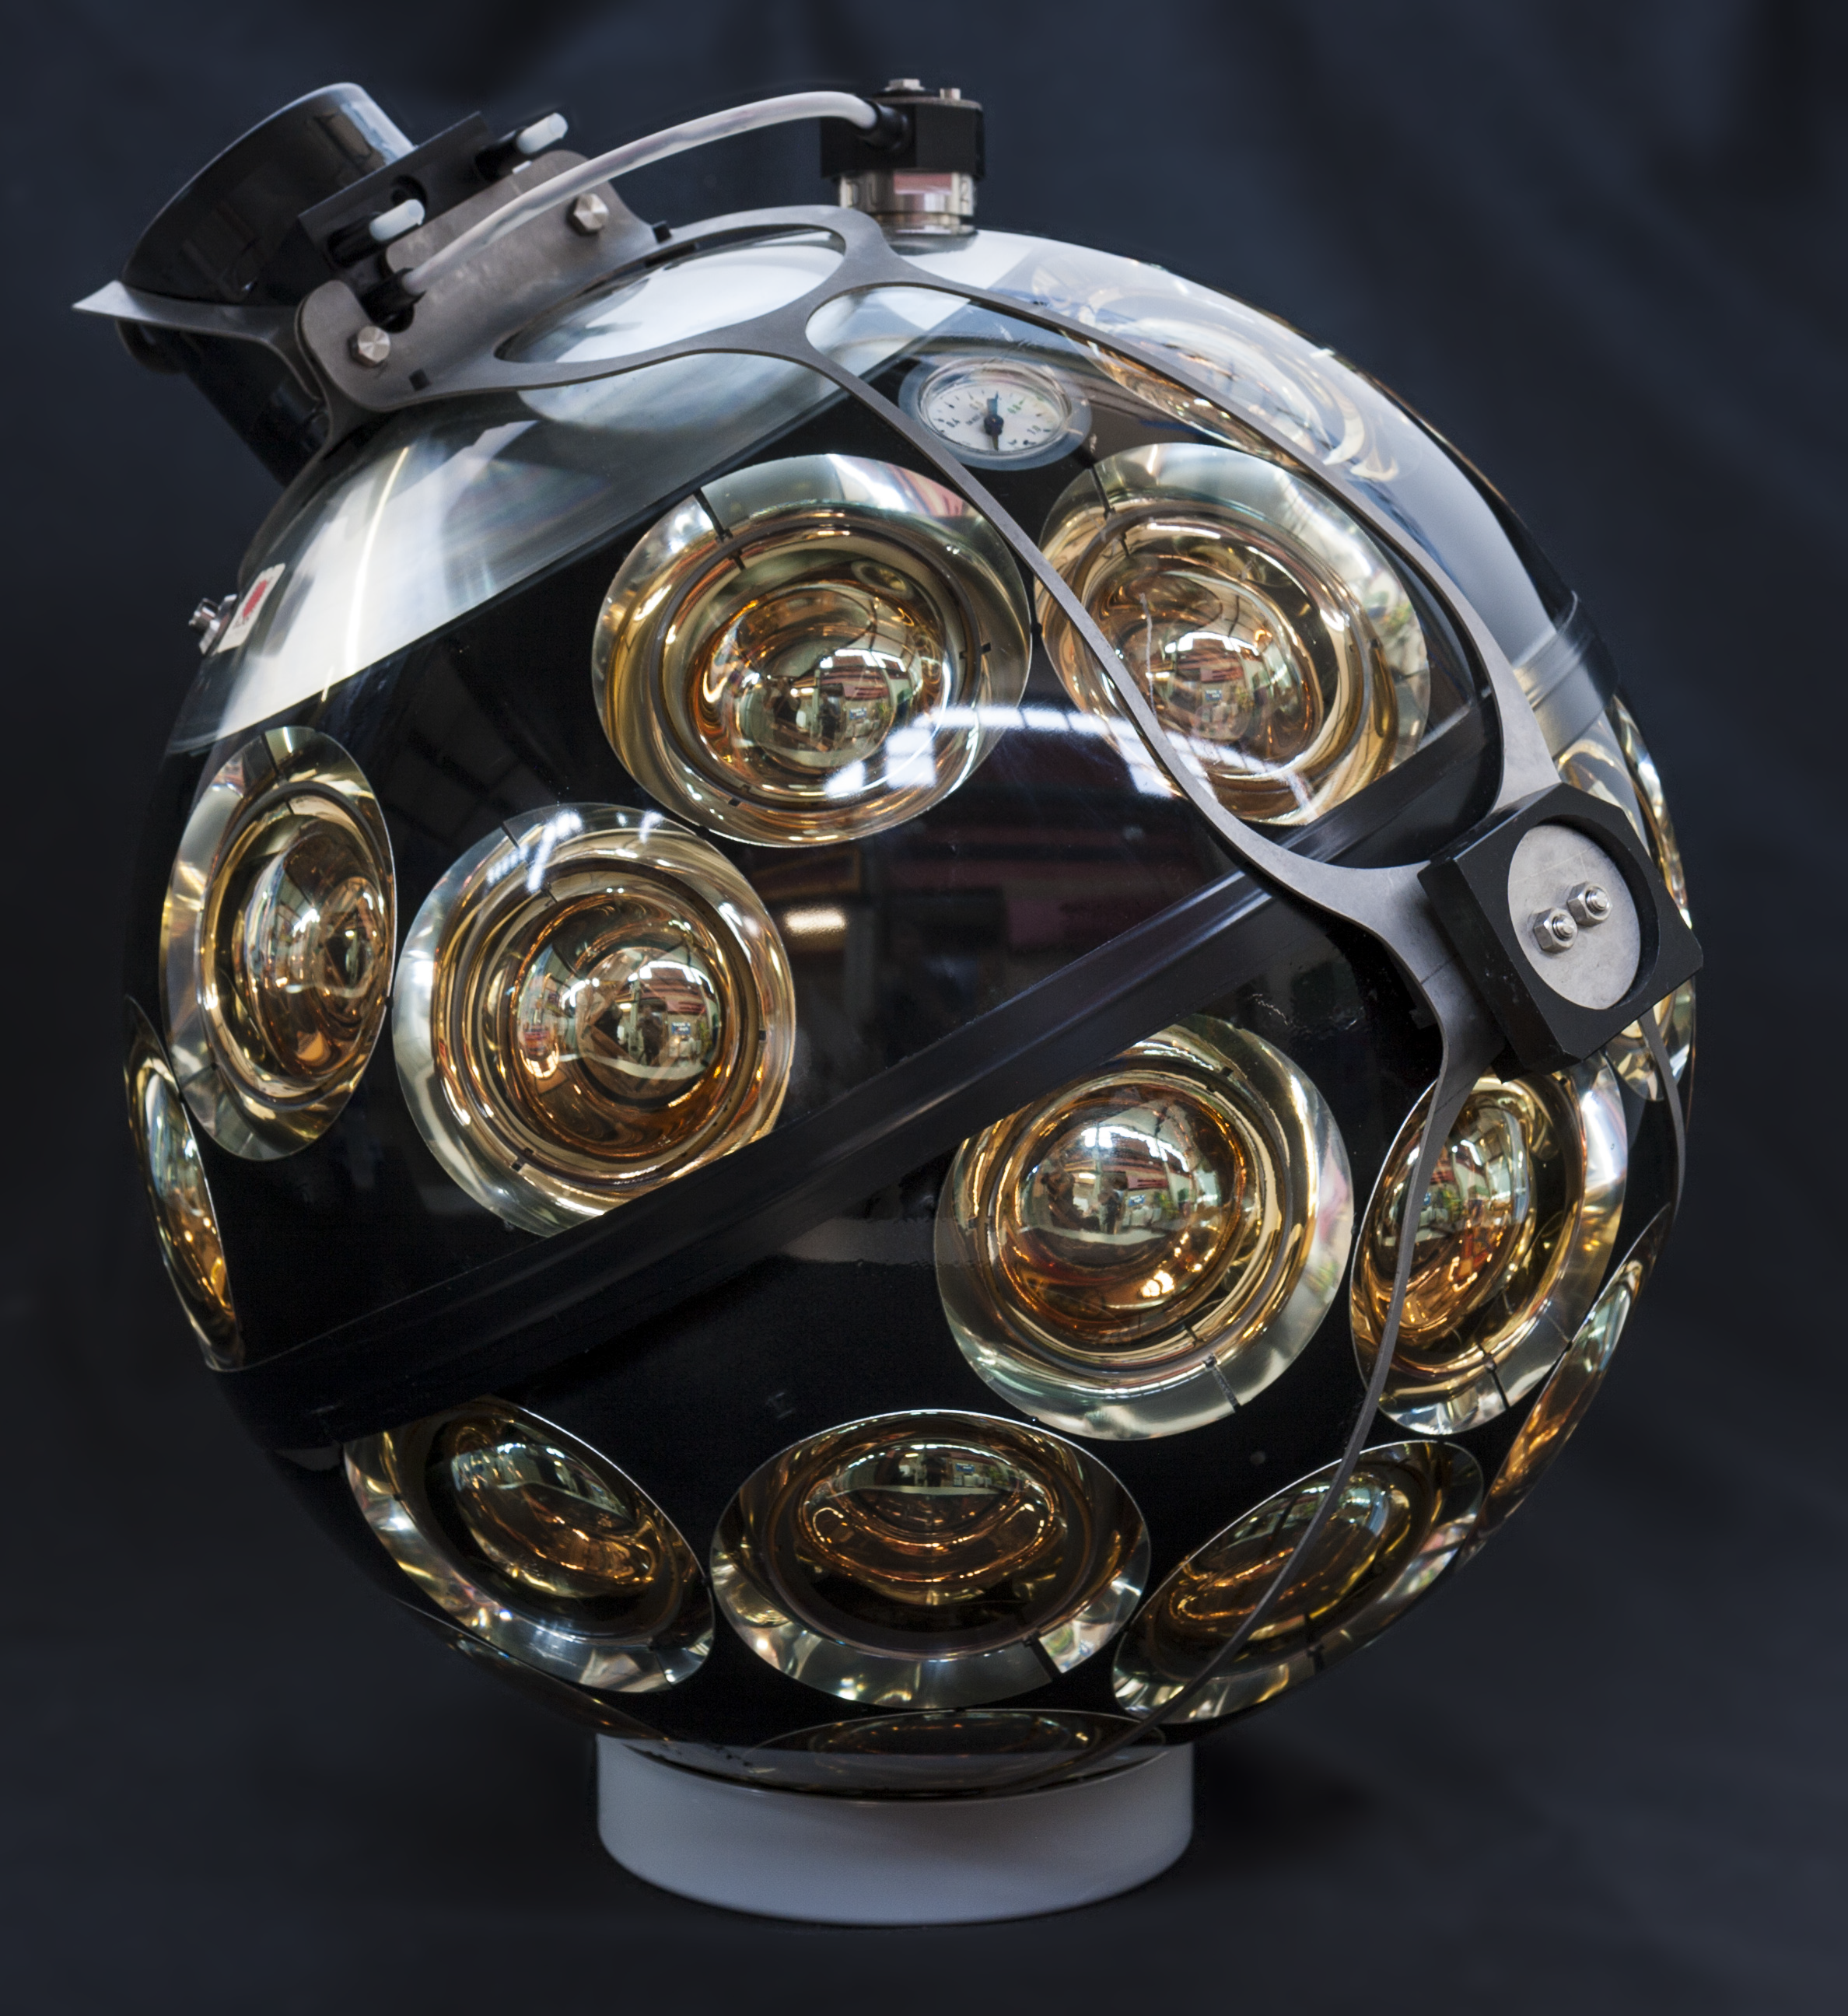
\includegraphics[width=\linewidth]{doms.png}
    \caption{An optical detector (DOM) \textit{source: https://www.km3net.org}}%
    \label{fig:doms}    
  \end{minipage}
\end{figure}

\section{Situation of Concern}
\label{sec:soc}

The ARCA telescope comprises of two ``blocks'' with a total volume of
$1km^{3}$. Each block consists of 115 spherical detector units (DOMs)
and each DOM consists of 31 Photo Multiplier Tubes (PMTs) in various
spacial arrangement. Figure \ref{fig:blocks} shows an artist's
impression of ARCA, figure \ref{fig:doms} depicts a DOM along with the
PMTs inside it. The PMTs are highly sensitive to light (photons), and
thus are used to detect the Cherenkov Radiation of neutrino particles.
The analog signal for all hits above a certain threshold are
digitized. This datapoint consists of a timestamp and the spatial
orientation of the DOM (ie. x,y,z coordinates). The digital signals
from all PMTs are arranged in 100ms ``timeslices'' and sent to the
on-shore facility for further processing \cite{aiello2019km3net}.

Unfortunately, there are several sources of noise (in this case, the
noise is other light sources), bioluminescense and decay of Potassium
40 ($^{40}K$) and atmospheric Muons being the primary sources
\cite{post2019km3nnet}. Due to the high level of noise, data is
generated at an extremely high rate of 25GB/sec
\cite{adrian2016letter} and must be filtered and selectively stored
for further analysis. The state of the art for this task are known as
``Event Trigger'' algorithms \cite{adrian2016letter,aiello2019km3net}
which can filter timeslices containing just noise thus only allowing
important timeslices containing neutrino hits to pass through. The
existing event trigger algorithms namely \emph{L1} and \emph{L2}
although able to conduct the filtration in near real, lack the ability
to do so with high accuracy thus often failing to save important
timeslices \cite{karas2019data}. Efforts have already been made to
improve the existing event trigger algorithms. Karas et al. (2019)
proposed and implemented a GPU powered pipeline which utilizes
correlation and graph community detection to identify time slices that
may contain neutrino hits whilst Post et al. (2019) suggests an
alternate using convolutional neural networks.

\section{User Requirements}
\label{sec:user-req}

The primary users of the ARCA are researchers who want to study high energy
particles from outer space. The stakeholders are all member institutes involved
in the project and by extension all scientists from these institutes who will
be working with the data collected.

The requirements of the primary users (and stakeholders) with respect to the
data acquisition pipeline are as follows.

\begin{enumerate}
  \item[\textbf{UR1}.]\textbf{The accuracy of filtration must be extremely high.}

    Time slices which are deemed important by event trigger algorithms
    are stored for further analysis and research. Failure to store
    timeslices containing information from neutrino events can lead to
    loss of important data and thus a poor quality of research. Since
    majority of the data generated is noise, the pipeline must be able
    to prevent storage of unnecessary timeslices containing only noise
    in the on-shore facility.

  \item[\textbf{UR2}.] \textbf{Filtration should occur in real time.}

    The state of the art event trigger algorithms are able to process
    data in real time. The proposed alternative ideally should
    maintain or improve upon it's predecessor's performance else
    provide a good trade off with data quality.

\end{enumerate}

\section{Research Question}
\label{sec:rqs}

This report presents research to improve upon \emph{The Karas
Pipeline}, a GPU pipeline proposed by Karas et al. (2019) to combat
the limitations of the L1 and L2 event trigger algorithms.
Specifically this project sought to answer the following research
questions.

\begin{enumerate}
  \item[\textbf{RQ1}.] \textbf{Can the existing GPU pipeline be improved using neural networks (NNs)?}

    Improvement may be achieved by reducing the processing time of the
    pipeline or improving the accuracy of identifying important
    timeslices. This project focuses on achieving improvement via
    accuracy and the task of validating the runtime performance of the
    methods proposed in this paper is left to a separate project.

    In order to answer \textbf{RQ1}, the following sub questions are
    formulated.

  \item[\textbf{RQ2.}] \textbf{Can the \emph{Hit Correlation Step} be replaced with a Multi Layer Perceptron?}

    The first step of The Karas Pipeline is the Hit Correlation Step,
    a novel trigger criterion which given a pair of points, can
    quantify the level of correlation amongst the points with an
    accuracy of 80\%. The first phase of this project focuses on
    achieving better accuracy to identify such ``causally related''
    points using a Multi Layer Perceptron (MLP).
    
  \item[\textbf{RQ3.}] \textbf{Can the \emph{Graph Community Detection Step} be replaced with a Graph Convolusional Neural Network?}

    The output of the Hit Correlation Step is used to create a graph
    structure where hits (of neutrino and noise) are represented as
    nodes connected with an undirected edge carrying the probability
    of correlation as its weight. The Constant Pots clustering
    algorithm, which operates on the principles of Graph Community
    Detection \cite{fortunato2010community}, is used to separate the
    graph into communities of neutrino and noise hits. The second
    phase of this project focuses on achieving a better accuracy for
    clustering neutrino and noise hits into separate communities in a
    given timeslice using Graph Convolusional Neural Networks (GCNs)
    \cite{kipf2016semi}.
\end{enumerate}

The following chapters of this report present the research efforts
carried out to improve The Karas Pipeline using Artificial Neural
Networks. In Chapter \ref{cha:data} the steps taken to prepare the
dataset used in this project is presented followed by its statistical
analysis and visual exploration. Since this research initiative is a
direct offshoot of the work previously conducted by Karas et al.
(2019), an overview of The Karas Pipeline is presented in Chapter
\ref{cha:karas-pipeline}. Chapters \ref{cha:mlp} and \ref{cha:gcn}
present detailed analysis of the neural networks created to replace
segments of The Karas Pipeline. Drawing from the results of the
replacement models, practical recommendations and directions for
further research are laid out in Chapter \ref{cha:rec}. This report is
intended for the primary users of ARCA with the hope to aid in the
development of the successor to the state of the art event trigger
algorithms. The report may also be used by deep learning practitioners
working in the field of neutrino detection. This report assumes the
reader posses a background in Computer Science or Artificial
Intelligence and thus is familiar with concepts such as statistics,
linear algebra and optimization. The reader is expected to have basic
understanding of the guiding principals of Deep Learning such as
Feed-Forward Neural Networks, backpropagation, binary classification
and model evaluation metrics.
